% !TeX spellcheck = en_EN-English

\section{Prediction of record cost}
\label{costPredImple}

As discussed in \ref{recCostPred} we would use MLP to predict cost of record. However since our goal is to predict future cost category of patient and not exact cost amount we decided to also predict cost category of record instead of it's precise cost.
\\

To assess how to split interval of possible costs into sub-intervals corresponding to each category with visualized costs of records from our training dataset in histogram. Resulting histogram can be see on Fig. \ref{fig:cost_hist} where y axis is linear while x axis is logarithmic as well as size of bins increase logarithmically, there we can see that most of records have cost between 0.1€ and 200€, so that's where we want most of cost categories to be. We decided to merge all cost under one euro into single category since even though they are numerous they have very small influence on total cost of patient in year. Then we split interval between 1 and 200 into 6 categories with increasing width, after that we group few outliers between 200 and 500 into one category and finally we give all outliers above 500 last category. This gave us 9 categories which are summarized in Tab. \ref{tab:cat_interval_record}.

\begin{figure}[!h]
	\centering
	
	% TODO image needs update with one computed from real training dataset
	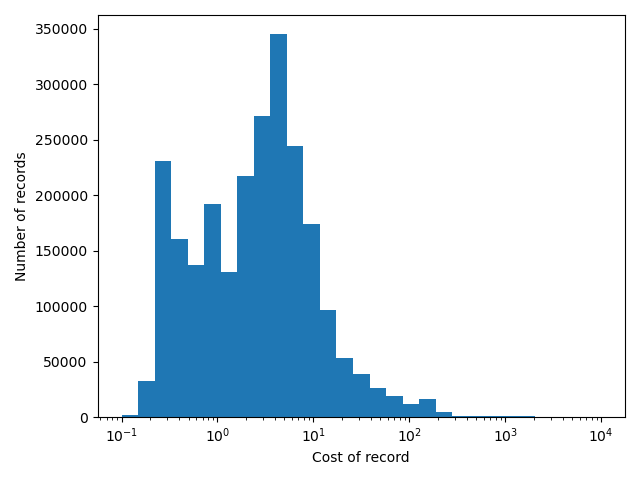
\includegraphics[width=0.8\textwidth]{images/cost_hist.png} 
	
	\caption{Histogram showing distribution of cost of records in training dataset.}
	\label{fig:cost_hist}
\end{figure} 

\begin{table}[!h]
	\centering
	\begin{tabular}{|l|l|}
		\hline
		Category  & Interval \\ \hline
		1 & $\interval[{0,1})$ \\ \hline
		2 & $\interval[{1,5})$ \\ \hline
		3 & $\interval[{5,10})$ \\ \hline
		4 & $\interval[{10,20})$ \\ \hline
		5 & $\interval[{20,50})$ \\ \hline
		6 & $\interval[{50,100})$ \\ \hline
		7 & $\interval[{100,200})$ \\ \hline
		8 & $\interval[{200,500})$ \\ \hline
		9 & $\interval[{500,\infty})$ \\ \hline
	\end{tabular}
	\caption{Intervals of cost for each category.}
	\label{tab:cat_interval_record}
\end{table}  

Model itself consist of input layer of size 196 (final size of our embedding) after that there are multiple linear layers with non-linear functions in-between. In then with get to final layer of size 9, so number of our categories, results of this final linear layer goes into softmax function to get transformed from resulting values into probabilities of each category. 
\\

We optimize multiple parameters of network itself as well few parameters important for training. From perspective of model itself we tried multiple number of layers so depths of model, as well as their size and non-linear functions in-between them. From training perspective tried three loss functions, more precisely we tried mean square loss, cross entropy loss and negative log likelihood loss, and multiple values for learning rate. For optimizer we choose Adam \cite{adam}.  
\\

Setting of parameters was done by training multiple models on smaller subset of dataset locally and then final model was trained on chosen parameters with complete dataset on server.